\section{Programming and interacting with the MCU}

\subsection{Setting up the project}

As mentioned in the introduction, you will not start from scratch. We provide you with a  baseline version of the code you need for this session. To ensure you have the latest version of the code, remind to \texttt{git pull} from the GitHub project repository and then open STM32CubeIDE. At the first launch of the IDE, it will prompt you to choose a workspace, you can either keep the default one or choose an alternative folder. In order to open the project in the IDE, click on \textbf{File} $\rightarrow$ \textbf{Open Projects from File System}. Then in the new window, click on \textbf{Directory} and choose the \path{mcu/} folder . Make sure that a project appears in the box below, select it if not selected. It should look as in \autoref{fig:import_ide}. Click on \textbf{Finish}. If you land on the welcome page, close the \textbf{Information Center} tab from the IDE. You should now see the \texttt{README.md} file and the \textbf{Project Explorer} tab on the left as in \autoref{fig:stm32cubeide}.

\begin{figure}[H]
    \centering
    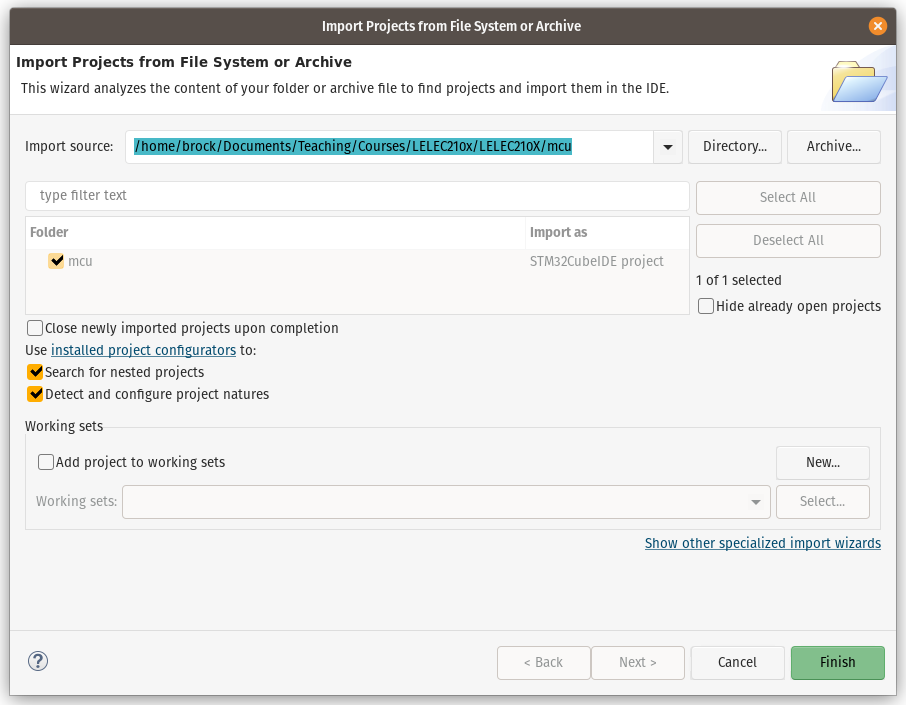
\includegraphics[width=.65\textwidth]{figures/import_ide.png}
    \caption{Open project from file system.}
    \label{fig:import_ide}
\end{figure}

\begin{figure}[H]
    \centering
    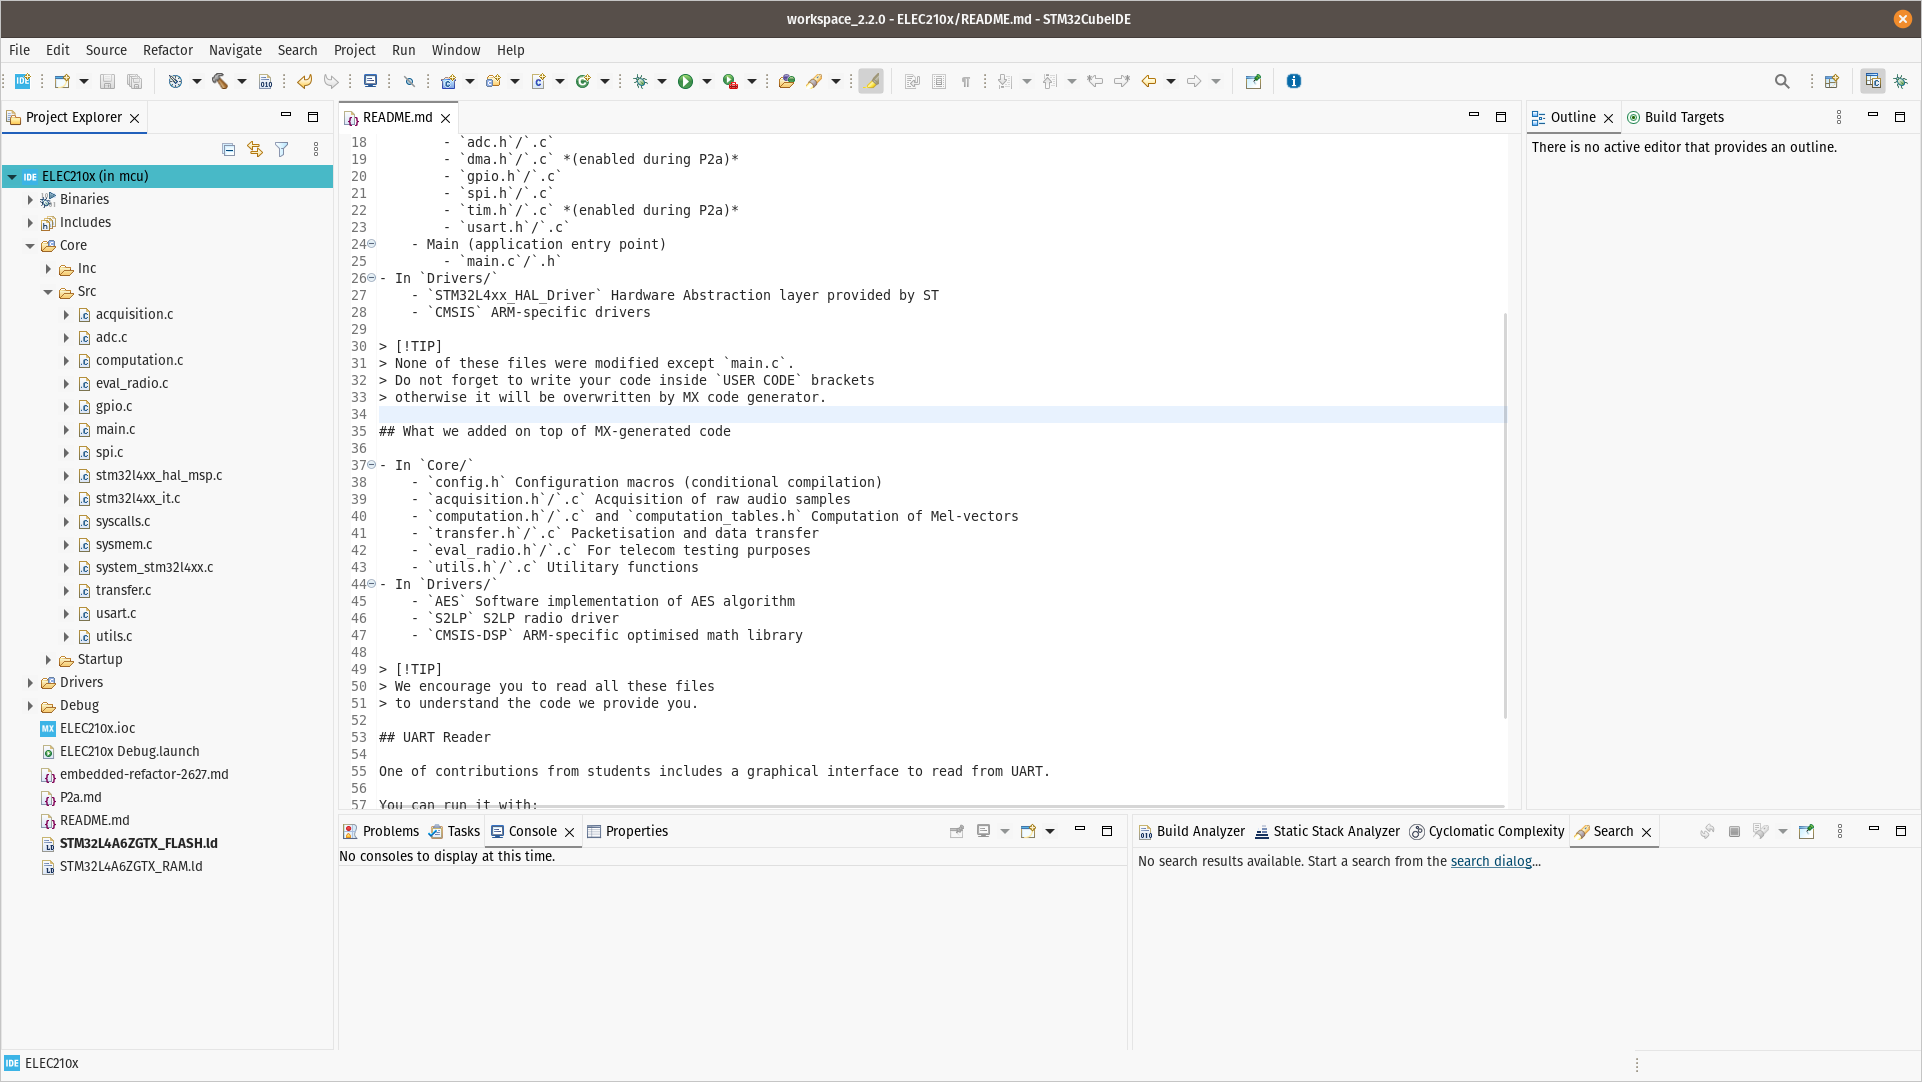
\includegraphics[width=.8\textwidth]{figures/stm32cubeide.png}
    \caption{STM32CubeIDE.}
    \label{fig:stm32cubeide}
\end{figure}

Skim through \texttt{README.md} to understand the source files structure. Double-click on \texttt{ELEC210x.ioc} to open it in STM32CubeMX. If it doesn't work, launch the app, search for the file and open it manually. If you are asked to continue with the old version or migrate to the new one, choose \textbf{Migrate}. The project should now be open in CubeMX as in \autoref{fig:stm32cubemx}.

\begin{bclogo}[couleur = gray!20, arrondi = 0.2, logo=\bcinfo]{STM32CubeMX}
STM32CubeMX is graphical tool provided by ST. It is a convenient way of configuring many hardware-related setting from the MCU. It generates source files that contain C code initializing the hardware as requested. We will use it in the project to configure the clocks, hardware peripherals and many other things.
\end{bclogo}

\begin{figure}[H]
    \centering
    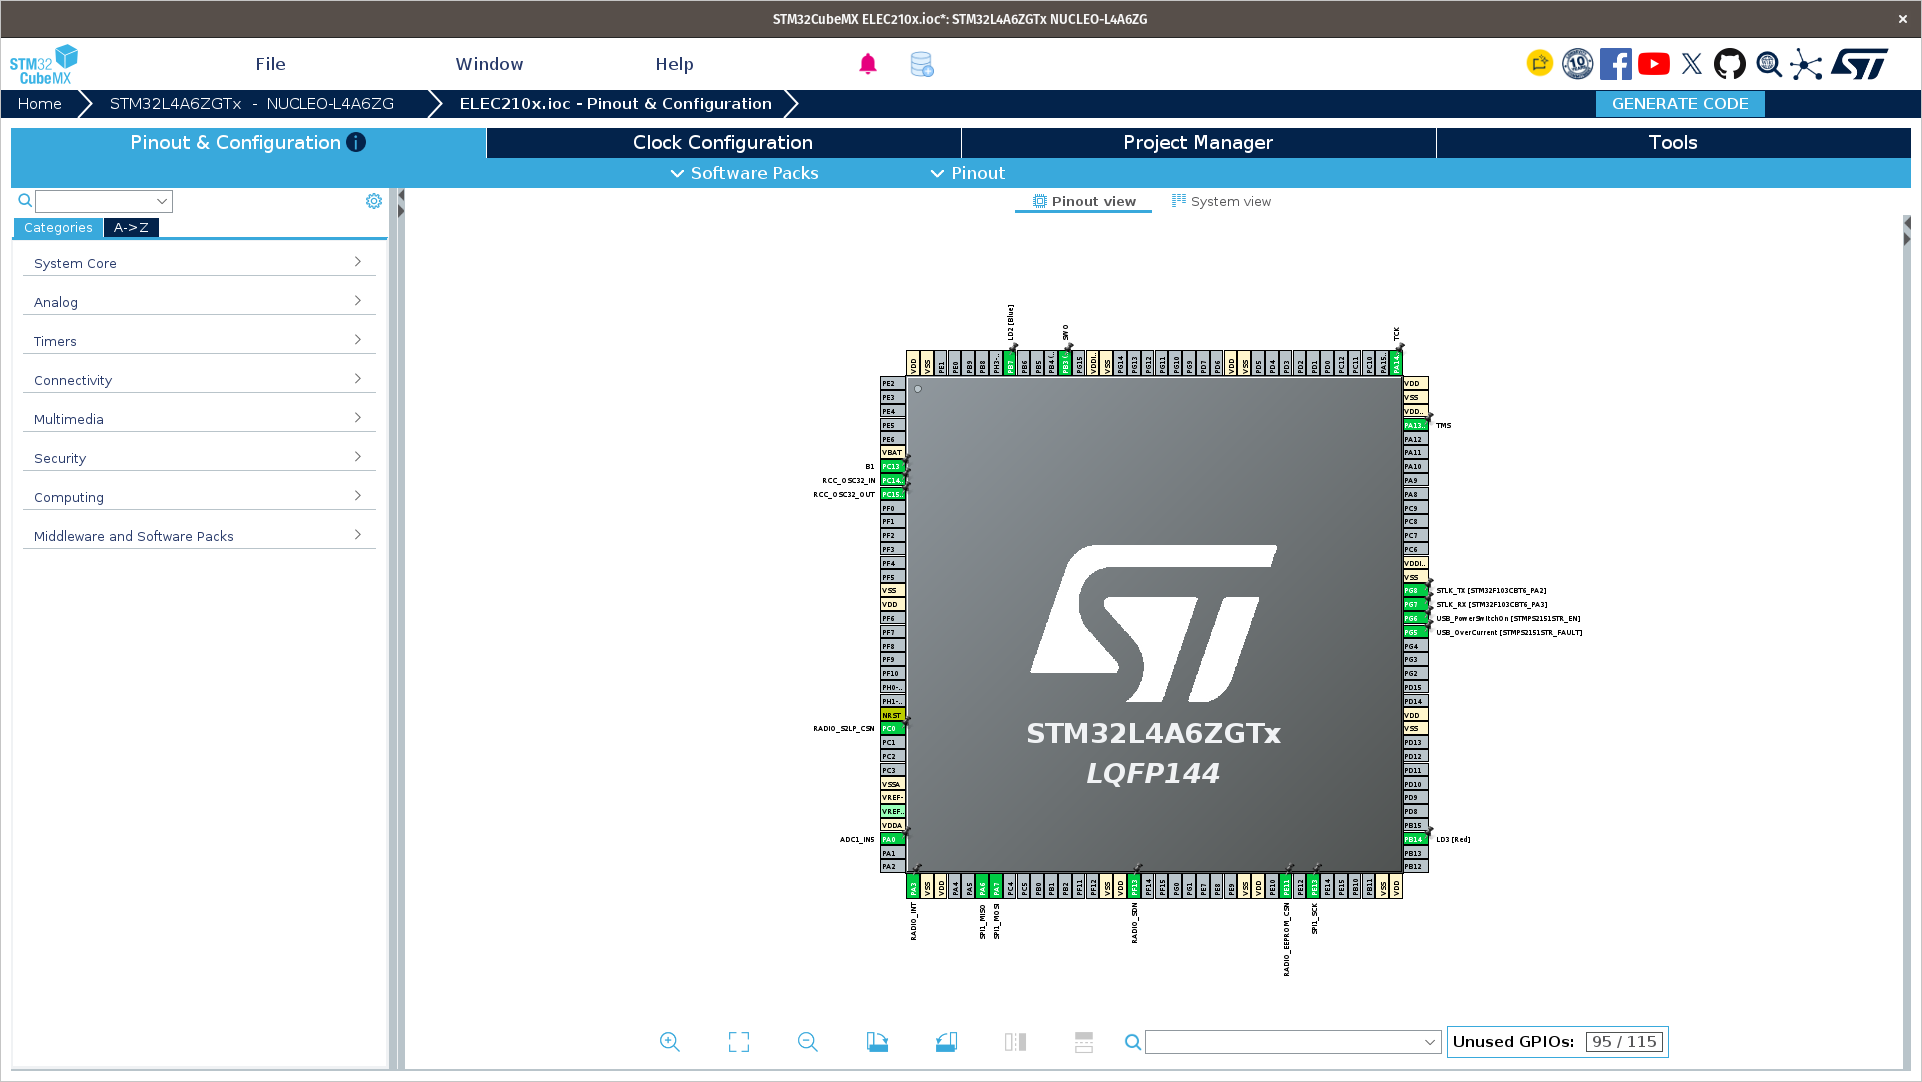
\includegraphics[width=.8\textwidth]{figures/stm32cubemx.png}
    \caption{STM32CubeMX.}
    \label{fig:stm32cubemx}
\end{figure}

Now, in order to compile the binaries for our specific MCU, you need to download the corresponding firmware package. Open \textbf{Help}$\rightarrow$ \textbf{Manage embedded software packages}, then in \textbf{STM32Cube MCU Packages} locate \textbf{STM32L4} and install the latest version available. It should look like \autoref{fig:mx_software_package}. Close the embedded software packages window and let MX generate the code using \textbf{the dedicated "GENERATE CODE" button} in the upper right corner, then close STM32CubeMX for now.

\begin{figure}[H]
    \centering
    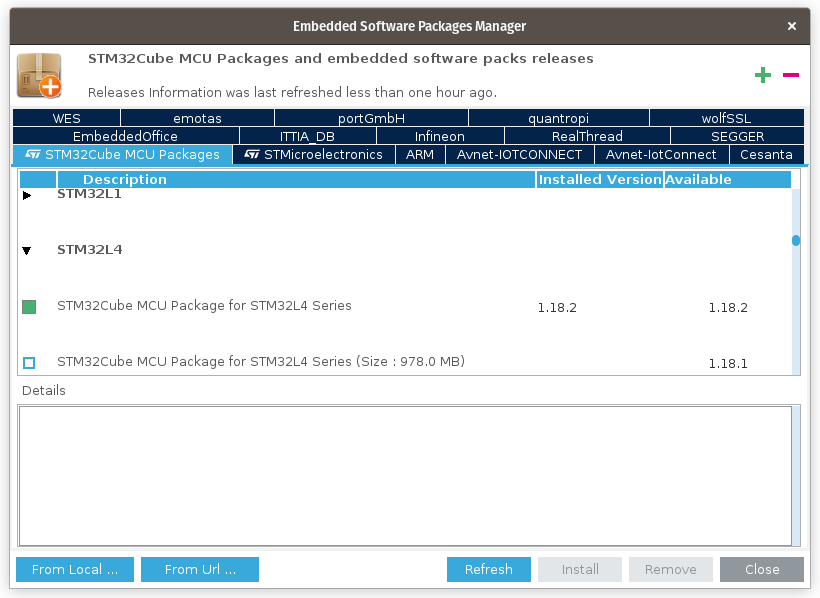
\includegraphics[width=.65\textwidth]{figures/mx_software_package.png}
    \caption{Embedded software packages manager.}
    \label{fig:mx_software_package}
\end{figure}

\subsection{Building the project and flashing the MCU}

STM32CubeIDE is not just a text editor, it comes with three essential tools :
\begin{enumerate}
    \item{\textbf{The builder}} or compiler comes as a preconfigured toolchain to cross-compile our C code into a binary specific to our MCU's architecture. Compile the project by clicking \textbf{the hammer-shaped button} of the IDE. You should not get any warning nor error at this point in the IDE's console at the bottom of the window.
    \item{\textbf{The flasher}} or programmer is used to write the generated binary to the flash memory of the MCU. Use \textbf{the green triangle "play" button} to flash the MCU. It actually triggers a project build then flash sequence. The first time you flash a project, you may be prompted to choose a configuration; keep the default and click \textbf{OK}. If you are prompted to \textbf{update the ST-LINK firmware}, press \textbf{Yes}, then \textbf{Open in update mode}, then \textbf{Upgrade}. When successfully updated, close the window and restart the flash procedure. You should see in the console that the download is verified successfully then the flasher shut down.
    \item{\textbf{The debugger}} is the third useful tool. It enables to follow the MCU's code execution in real time and inspect the register's content. More on that comes at the end of this session. 
\end{enumerate}

\begin{bclogo}[couleur = gray!20, arrondi = 0.2, logo=\bcinfo]{ST-Link programmer}
The ST-Link is a programmer and debugger. It provides the connection between your computer and the MCU on the board. The MCU is connected to the ST-LINK through an interface named JTAG. In the case of the Nucleo MCU board, a dedicated ST-Link is soldered onto the board and is always connected to the MCU. It also serves as an USB to UART adapter.
\end{bclogo}

\subsection{Reading and understanding the code}

Open the file \textbf{ELEC210x/Core/Src/main.c} and scroll to the \texttt{main()} function which is the application entry point. In embedded systems, it is usually divided in two steps.
\begin{enumerate}
    \item{The initialisation} or setup where the hardware (clocks, peripherals, etc.) is configured according to what CubeMX generated.
    \item{The infinite loop} or main loop, from which the application should never escape otherwise the CPU would execute random pieces of code as it cannot be stopped like a process.
\end{enumerate}

You surely have noticed our main loop is empty. That's because we use \textbf{interrupt-based programming} to execute tasks triggered by external events (e.g. user button press) or internal events (e.g. timer period elapsed).

Take a look at \texttt{HAL\_GPIO\_EXTI\_Callback()}, it is called by the \textbf{interrupt software routine (ISR)} whenever an external interrupt is triggered. Read and understand the code executed when the user button is pressed.

\begin{bclogo}[couleur = gray!20, arrondi = 0.2, logo=\bcinfo]{Preprocessor and macro language}
In this project, we make extensive use of macros (\texttt{\#define}, etc.) and conditionals (\texttt{\#if}, \texttt{\#else}, \texttt{\#endif}, \texttt{\#ifdef}, etc.) to make the code versatile. The preprocessor is executed first in the compilation chain and adapts the source code fed to the compiler based on these macro instructions. For more details, check out \url{https://gcc.gnu.org/onlinedocs/cpp/index.html#SEC_Contents}, mainly \textbf{Macros} and \textbf{Conditionals}.

Check out \textbf{Core/Inc/config.h} to find configuration macros for application parameters and conditional compilation.
\end{bclogo}

\begin{bclogo}[couleur = gray!20, arrondi = 0.2, logo=\bcinfo]{Hardware Abstraction Layer (HAL)}
The MCU and its peripherals are controlled by memory-mapped registers. That is, in order to control them, bytes must be read or written at a specific memory address (the address and value written determine the action performed -- find these in the reference manual of the MCU).
ST provides a HAL, which is a set of functions that abstract sequence of such reads and writes. We strongly recommend you to use it (see the HAL description document). There are two kind of HAL functions provided: the standard ones and the low level (LL) ones. The standard ones are high-level and application-oriented, while the LL are faster but less easy to use. We recommend you to stick to the standard HAL functions (without "\_LL\_").
\end{bclogo}

\begin{bclogo}[couleur = gray!20, arrondi = 0.2, logo=\bcinfo]{Callback implementation}
You may have noticed that callbacks such as \texttt{HAL\_GPIO\_EXTI\_Callback()} are already defined in the HAL library, with the \texttt{\_\_weak\_\_} attribute. Weak functions are designed to be overwritten by the user's implementation. By redefining the function with the same signature (without the attribute), you effectively implement the already defined function.

\textit{Tip:} To quickly find the definition of any variable or function, use \texttt{ctrl+click} in the IDE. Many other shortcuts are useful, do not hesiste to look for them.
\end{bclogo}

\subsection{Interacting with the embedded system}

\paragraph{Lighting an LED}
Until now, you have no idea whether the program you flashed is actually working or not. A convenient way of getting feedback from the system is to blink an LED when doing tasks. Use \texttt{HAL\_GPIO\_WritePin(LD2\_GPIO\_Port, LD2\_Pin, GPIO\_PIN\_SET)} to light on the blue user LED during the acquisition, then light it off by writing \texttt{GPIO\_PIN\_RESET} to the pin once the acquisition is finished, before printing the raw samples. Build and flash, then observe the LED lighting on during the acquisition.

\paragraph{Retrieving printf output}

The last task performed in the callback procedure is to print the acquired raw audio samples. \texttt{print\_raw\_samples()} formats the samples as a string of hexadecimal values and prints it through UART. On your host computer, run \texttt{uv run uart-reader} to launch our custom UART reader graphical application. Select \textbf{STM32 STLink} in the \textbf{Serial Port} drop menu, then click \textbf{Connect} to monitor the UART stream. Press \textbf{the black (reset) button}, the MCU greets you in the console. Press \textbf{the blue (user) button}, a window will open with the plot of the raw samples once the MCU has finished acquiring and printing them. For now, observe and comment the \textbf{audio signal plot} only, not on the FFT plot.

\begin{bclogo}[couleur = gray!20, arrondi = 0.2, logo=\bcinfo]{Printing to the console}
We have defined a macro function \texttt{DEBUG\_PRINT()} that encapsulates \texttt{printf()} to allow conditional compilation and save resources (CPU cycles and code size) if the printing feature is not required (check out \textbf{Core/Inc/config.h}).

In \textbf{Core/Src/utils.c}, we redirect the printf function to UART. The ST-Link makes the bridge between the MCU's UART and the host computer's USB. UART is a serial communication bus whose speed is set by the \textbf{baud rate} corresponding to the number of bits sent per second.
\end{bclogo}

\begin{bclogo}[couleur = gray!20, arrondi = 0.2, logo=\bcquestion]{Raw samples value and ADC resolution}
What is the format of the value you get from the ADC ? To how many bits does the ADC quantize its input voltage ? How many quantificition levels does that represent and what is thus the voltage resolution ? Describe the audio signal you observe.

\textit{Tip:} You can look for information in the MCU datasheet available on Moodle, the ADC configuration in CubeMX and the schematic in the \textit{Guide - how to use the boards} on Moodle in the technical resources.
\end{bclogo}

\begin{bclogo}[couleur = gray!20, arrondi = 0.2, logo=\bcquestion]{Acquisition frequency and transfer duration}
\begin{itemize}
    \item By observing the blinking LED, can you approximate the time taken by the MCU to acquire 10 000 samples ? Is the sampling frequency controlled ? What does the sampling frequency depends on in the current implementation ? What problem or drawback do you spot in the current implementation, regarding the objective of acquiring audio samples ? 
    \item Can you approximate the duration the MCU takes to print the acquired raw samples ? What limits the speed of data transfer ? How can you theoritecally compute the time it takes to print the raw sample string through UART ? Does it match what you observe ?
\end{itemize}
\end{bclogo}

\newpage

\section{Using a timer to control the sampling frequency}

Instead of launching ADC conversions in software, we will now configure a timer to trigger the acquisition at a regular rate (the sampling frequency). \textbf{Open STM32CubeMX} by clicking on the \texttt{.ioc} file in the project explorer. Understand and follow these instructions to configure the timer and the ADC.
\begin{enumerate}
    \item In the \textbf{Pinout \& Configuration} tab (the default open one), click on \textbf{Timers} $\rightarrow$ \textbf{TIM3} to open its configuration tab ;
    \item Choose \textbf{Clock Source : Internal clock} in the \textbf{Mode} panel ;
    \item Under \textbf{Configuration} $\rightarrow$ \textbf{Parameter Settings}, set
        \begin{enumerate}
            \item \textbf{Prescaler} to \textbf{47} ;
            \item \textbf{Counter Period} to \textbf{99} ;
            \item \textbf{Trigger Event Selection TRGO} to \textbf{Update Event} ;
            \item Leave the other parameters to their default value.
        \end{enumerate}
    \item Now search for \textbf{Analog} $\rightarrow$ \textbf{ADC1} in the left panel and open the ADC tab;
    \item Under \textbf{Configuration} $\rightarrow$ \textbf{Parameter Settings} $\rightarrow$ \textbf{ADC\_Regular\_ConversionMode}, set \textbf{External Trigger Conversion Source} to \textbf{Timer 3 Trigger Out Event}. Leave the other parameters to their default or already configured value ;
    \item Generate the code by clicking on the dedicated button and close CubeMX.
\end{enumerate}

\begin{bclogo}[couleur = gray!20, arrondi = 0.2, logo=\bcattention]{STM32CubeMX code generator}
When modifying your code, make sure to modify only the code that is between a \texttt{USER CODE BEGIN} and \texttt{USER CODE END} (do not modify these comments). These parts are the only ones not overwritten by CubeMX code generator, therefore preserving the changes you have implemented.
\begin{lstlisting}
  /* USER CODE BEGIN xxx */
     // insert your code here
  /* USER CODE END xxx */
\end{lstlisting}
\end{bclogo}

You also need to change the code to correspond to the new configuration. Implement the following pseudo-code as the acquisition procedure.
\begin{lstlisting}[columns=fullflexible]
Start ADC
Start timer
Loop 10000 times:
    Wait for conversion
    Read and store acquired value
Stop timer
Stop ADC
\end{lstlisting}

\begin{bclogo}[couleur = gray!20, arrondi = 0.2, logo=\bcattention]{Tips for implementation}
Use the corresponding HAL functions provided by ST:\\
\texttt{HAL\_TIM\_Base\_Start()} and \texttt{HAL\_TIM\_Base\_Stop()} for the timer, and the ones we already used for the ADC.

You will need to use the timer handle \texttt{htim3} to use the HAL functions. Look at line 76 and copy it for the timer. The \texttt{extern} keyword means the variable is declared in another source file and we simply want to make it reachable in this file. Usually, variables are defined in \texttt{.c} files. If they are intented to be used elsewhere, the corresponding \texttt{.h} makes it explicit by declaring them \texttt{extern}. Note that it is not strictly necessary as the \texttt{.h} file makes no use of the variable, it's simply for human-readability and understandability.
\end{bclogo}

\begin{bclogo}[couleur = gray!20, arrondi = 0.2, logo=\bcquestion]{Timer frequency}
\begin{itemize}
    \item Do you understand how the timer works ? What are the prescaler and the counter period parameters ? In what situation would a prescaler be required ?
    \item How can you compute the timer update event frequency $f_{update}$ based on the prescaler value $PSC$, the counter period $ARR$ (also called auto-reload register) and the source clock frequency $f_{src}$ ? The targetted sampling frequency is 10kHz, does your computation match ? \textit{Hint:} Check out the \textbf{Clock Configuration} tab in CubeMX to find the timer's input clock frequency.
    \item Write down or keep that equation in mind, it will be useful in the future to correctly reconfigure the timer if you change its input clock frequency.
\end{itemize}
\end{bclogo}

\begin{bclogo}[couleur = gray!20, arrondi = 0.2, logo=\bcquestion]{Analog front-end (AFE) and acquired audio signal}
The analog front-end is composed of the audio input (jack or microphone), the amplifier and the filter and is located on the custom (green) board. You can find the schematic in the \textit{Guide - how to use the board} in the technical resources on Moodle. We strongly advise you to read this document when you have the time as it contains a lot of useful information.
\begin{itemize}
    \item Draw a block diagram of the AFE and quantify the main block parameters (e.g. voltage swing, gain, cut-off frequencies, etc.) based on the the component values.
    \item Which important criterion should be respected regarding the signal spectrum and the sampling frequency ? Is it the case ? What happens if not ?
    \item What is the voltage swing you expect at the input of the ADC, knowing that the microphone's output AC component may vary from $\approx$10mV to $\approx$200mV depending on the sound level (the numbers are based on the microphone datasheet available on Moodle) ? How can you compute the measured voltage based on the acquired ADC value or the other way around ? Does it match what you observe in the audio signal plots ?
    \item Try to whistle a constant tone near the microphone while acquiring samples, or use an online tone generator on your computer and play it or feed it through jack. What are your observations on the audio signal and FFT plots ?
\end{itemize}
In uart-reader, you can save the recorded audio signal to a \texttt{.wav} file and play it on your computer. Crazy, right ?
\end{bclogo}

\newpage

\section{Debugging your code}

If you already got involved in some kind of programming, you know that it never goes as expected at the first shot (at least, not often). You therefore need to start debugging your code to understand where things go wrong and fix the issue. Of course, you can use \texttt{printf}'s to debug your code. However, as it has been said before, the ST-Link is also a debugger. We can halt the MCU at a specific line of code, look at the values of variables and registers, advance in the code step by step, and many others functionalities. To access the debugger mode, you need to launch your code with the \textbf{"green bug" button} just on the left of the run button you use for normal flashing. You can switch to the debugger perspective as proposed by the IDE.
Next, we detail how to use the debugger functionalities :
\begin{itemize}
    \item \textbf{Breakpoints} are lines or code that trigger a halt on the MCU. They allow to stop the MCU at a specific line of code and observe its state. To set up a breakpoint, simply double click on the line number where you want to put your breakpoint. The MCU will halt before the execution of this line. You should see a small blue dot at the left of the line number as in line 147 of \autoref{fig:breakpoint}

    \begin{figure}[H]
    \centering
    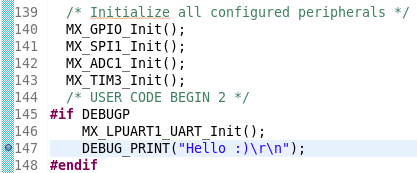
\includegraphics[width=.4\textwidth]{figures/breakpoint.png}
    \caption{Breakpoints in the IDE.}
    \label{fig:breakpoint}
    \end{figure}

    \item \textbf{Step by step execution} of the code is performed thanks to the buttons in the toolbar as in \autoref{fig:debugtools}. The play and pause buttons allow starting and stopping the MCU, and the 3 rightmost buttons allow advancing step by step in the code.

    \begin{figure}[H]
    \centering
    
\includegraphics[width=.3\textwidth]{figures/debugging.png}
    \caption{Debugging toolbar.}
    \label{fig:debugtools}
    \end{figure}

    \item \textbf{Variable values } can be observed in the right panel. The \textbf{Variables} tab contains the declared variables and their corresponding value at the breakpoint. It allows you to inspect what is happening during the code execution. Setup a breakpoint just before entering the acquisition loop and observe the variables as in \autoref{fig:debug_variables}.

    \begin{figure}[H]
    \centering
    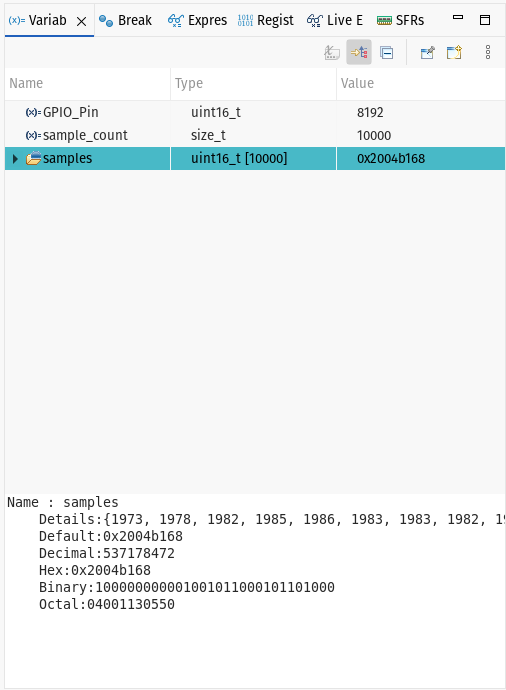
\includegraphics[width=.4\textwidth]{figures/debugger_variables.png}
    \caption{Debugger variables.}
    \label{fig:debug_variables}
    \end{figure}

\end{itemize}

When you debug real-time software, don't forget that when reaching a breakpoint, your code is not real-time anymore ! A few \texttt{printf} can also be helpful\dots

\begin{bclogo}[couleur = gray!20, arrondi = 0.2, logo=\bcattention]{Don't abuse of \texttt{printf}s}
Be aware that the \texttt{printf} function is hungry in CPU cycles. If you decide to print too much information, you might miss real-time constraints.
\end{bclogo}
